\begin{figure}[htbp]
\centering
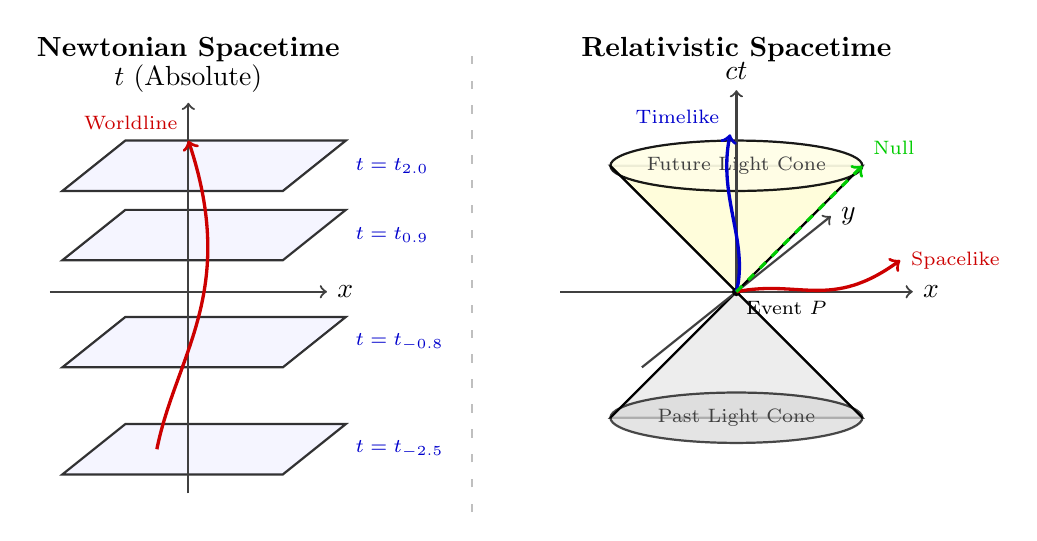
\begin{tikzpicture}[scale=0.8]
  % ----- Left: Newtonian Spacetime -----
  \begin{scope}[shift={(-4.5, 0)}]
    \node[above, font=\bfseries] at (0, 3.5) {Newtonian Spacetime};
    
    % Planes of absolute simultaneity
    \foreach \y in {-2.5, -0.8, 0.9, 2.0} {
      \draw[thick, fill=blue!5, opacity=0.8] (-2, \y-0.4) -- (1.5, \y-0.4) -- (2.5, \y+0.4) -- (-1, \y+0.4) -- cycle;
      \node[right, blue!80!black, font=\scriptsize] at (2.5, \y) {$t = t_{\y}$};
    }
    
    % Axes
    \draw[->, thick, darkgray] (0,-3.2) -- (0, 3.0) node[above, text=black] {$t$ (Absolute)};
    \draw[->, thick, darkgray] (-2.2,0) -- (2.2, 0) node[right, text=black] {$x$};
    
    % Particle worldline
    \draw[very thick, red!80!black, ->] (-0.5, -2.5) .. controls (-0.2, -1) and (0.8, 0) .. (0.0, 2.4) node[above left, font=\scriptsize] {Worldline};
  \end{scope}

  % ----- Divider -----
  \draw[thick, loosely dashed, gray!50] (0, -3.5) -- (0, 4);

  % ----- Right: Relativistic Spacetime -----
  \begin{scope}[shift={(4.2, 0)}]
    \node[above, font=\bfseries] at (0, 3.5) {Relativistic Spacetime};
    
    % Past Light Cone
    \draw[thick, fill=gray!20, opacity=0.7] (-2,-2) -- (0,0) -- (2,-2) -- cycle;
    \draw[thick, fill=gray!30, opacity=0.7] (0,-2) ellipse (2 and 0.4);
    \draw[thick] (-2,-2) -- (0,0) -- (2,-2);
    
    % Axes (drawn behind future cone, over past cone)
    \draw[->, thick, darkgray] (-2.8,0) -- (2.8, 0) node[right, text=black] {$x$};
    \draw[->, thick, darkgray] (-1.5,-1.2) -- (1.5, 1.2) node[right, text=black] {$y$};
    
    % Future Light Cone
    \draw[thick, fill=yellow!20, opacity=0.7] (-2,2) -- (0,0) -- (2,2) -- cycle;
    \draw[thick, fill=yellow!10, opacity=0.9] (0,2) ellipse (2 and 0.4);
    \draw[thick] (-2,2) -- (0,0) -- (2,2);
    \draw[->, thick, darkgray] (0,0) -- (0, 3.2) node[above, text=black] {$ct$};
    
    % Labels for regions
    \node[font=\scriptsize, darkgray] at (0, -2) {Past Light Cone};
    \node[font=\scriptsize, darkgray] at (0, 2) {Future Light Cone};

    % Origin Event
    \fill[black] (0,0) circle (2pt) node[below right, font=\scriptsize] {Event $P$};

    % Causal Structure Worldlines
    % Timelike
    \draw[very thick, blue!80!black, ->] (0,0) .. controls (0.2, 0.8) and (-0.3, 1.5) .. (-0.1, 2.5) node[above left, font=\scriptsize] {Timelike};
    % Spacelike
    \draw[very thick, red!80!black, ->] (0,0) .. controls (1, 0.2) and (1.5, -0.3) .. (2.6, 0.5) node[right, font=\scriptsize] {Spacelike};
    % Null (on the cone)
    \draw[very thick, green!80!black, dashed, ->] (0,0) -- (2, 2) node[above right, font=\scriptsize] {Null};
  \end{scope}

\end{tikzpicture}
\caption{Comparison between Newtonian absolute spacetime and the causal structure of Minkowskian spacetime. The right panel illustrates the past and future light cones of an arbitrary event $P$, distinguishing between timelike, spacelike, and null worldlines.}
\label{fig:spacetime_comparison}
\end{figure}


\begin{figure}[htbp]
\centering
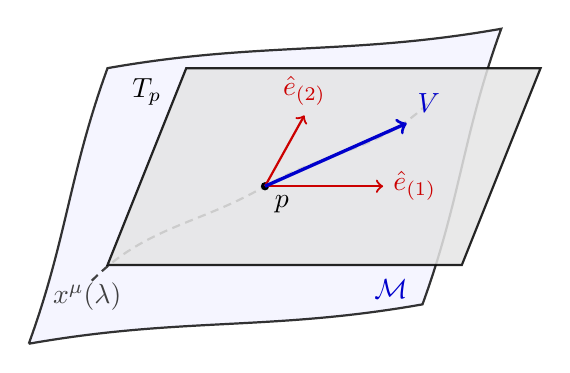
\begin{tikzpicture}[scale=1.0]
  % Define the center point p
  \coordinate (P) at (3, 2);

  % Draw the curved manifold (surface M)
  \draw[thick, fill=blue!5, opacity=0.8] 
    (0,0) to[out=10, in=190] (5,0.5) 
          to[out=70, in=250] (6,4) 
          to[out=190, in=10] (1,3.5) 
          to[out=250, in=70] (0,0);
  \node[blue!80!black] at (4.6, 0.7) {$\mathcal{M}$};

  % Draw a curve x^\mu(\lambda) on the manifold passing through p
  \draw[thick, densely dashed, darkgray] 
    (0.8, 0.8) to[out=45, in=210] (P) to[out=30, in=230] (5.2, 3.2);
  \node[darkgray, above left] at (1.3, 0.3) {$x^\mu(\lambda)$};

  % Draw the tangent plane T_p at point p
  \draw[thick, fill=gray!20, opacity=0.85] 
    (1, 1) -- (5.5, 1) -- (6.5, 3.5) -- (2, 3.5) -- cycle;
  \node at (1.5, 3.2) {$T_p$};

  % Mark the point p
  \fill[black] (P) circle (1.5pt) node[below right] {$p$};

  % Basis vectors e_(\mu) on the tangent plane
  \draw[->, thick, red!80!black] (P) -- ++(1.5, 0) node[right] {$\hat{e}_{(1)}$};
  \draw[->, thick, red!80!black] (P) -- ++(0.5, 0.9) node[above] {$\hat{e}_{(2)}$};

  % Tangent vector V^\mu = dx^\mu / d\lambda
  \draw[->, very thick, blue!80!black] (P) -- ++(1.8, 0.8) node[above right] {$V$};

\end{tikzpicture}
\caption{Geometric representation of a differentiable manifold $\mathcal{M}$. A parameterized curve $x^\mu(\lambda)$ passes through a point $p$. The tangent vector $V^\mu$ to the curve resides in the local tangent space $T_p$, which is spanned by the coordinate basis vectors $\hat{e}_{(\mu)}$.}
\label{fig:tangent_space}
\end{figure}


\begin{figure}[htbp]
\centering
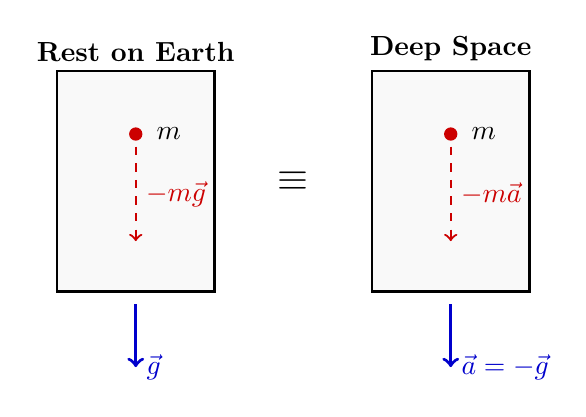
\begin{tikzpicture}[scale=0.8]
  % Left Box: Gravitational Field
  \draw[thick, fill=gray!5] (0,0) rectangle (2.5, 3.5);
  \node[above, font=\bfseries] at (1.25, 3.5) {Rest on Earth};
  \draw[->, very thick, blue!80!black] (1.25, -0.2) -- (1.25, -1.2) node[right] {$\vec{g}$};
  \fill[red!80!black] (1.25, 2.5) circle (3pt) node[right=4pt, text=black] {$m$};
  \draw[->, thick, dashed, red!80!black] (1.25, 2.3) -- (1.25, 0.8) node[midway, right] {$-m\vec{g}$};
  \draw[thick] (0.2, 0) -- (2.3, 0); % Floor emphasis

  % Right Box: Uniform Acceleration
  \begin{scope}[shift={(5,0)}]
    \draw[thick, fill=gray!5] (0,0) rectangle (2.5, 3.5);
    \node[above, font=\bfseries] at (1.25, 3.5) {Deep Space};
    \draw[->, very thick, blue!80!black] (1.25, -0.2) -- (1.25, -1.2) node[right] {$\vec{a} = -\vec{g}$};
    \fill[red!80!black] (1.25, 2.5) circle (3pt) node[right=4pt, text=black] {$m$};
    \draw[->, thick, dashed, red!80!black] (1.25, 2.3) -- (1.25, 0.8) node[midway, right] {$-m\vec{a}$};
    \draw[thick] (0.2, 0) -- (2.3, 0); % Floor emphasis
  \end{scope}

  % Equivalence symbol
  \node[font=\Large\bfseries] at (3.75, 1.75) {$\equiv$};
\end{tikzpicture}
\caption{Illustration of the Einstein Equivalence Principle. The local physical experiences of an observer resting in a uniform gravitational field $\vec{g}$ (left) are entirely indistinguishable from those of an observer in a uniformly accelerated reference frame with acceleration $\vec{a} = -\vec{g}$ in deep space (right).}
\label{fig:equivalence_principle}
\end{figure}


\begin{figure}[htbp]
\centering
\begin{minipage}{0.48\textwidth}
\centering
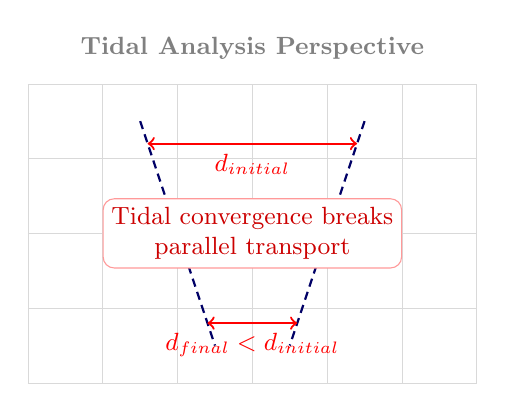
\begin{tikzpicture}[scale=0.95]
  % ----- Left Side: Tidal Analysis Grid -----
  % Rigid Cartesian Grid
  \draw[step=1cm, gray!30, very thin] (-3, 0) grid (3, 4);
  \node[gray, above, font=\bfseries\small] at (0, 4.2) {Tidal Analysis Perspective};

  % Falling paths (dashed trajectories)
  \draw[thick, blue!40!black, densely dashed] (-1.5, 3.5) -- (-0.5, 0.5);
  \draw[thick, blue!40!black, densely dashed] (1.5, 3.5) -- (0.5, 0.5);

  % Tidal effect annotations
  \draw[<->, thick, red] (-1.4, 3.2) -- (1.4, 3.2) node[midway, below, font=\small] {$d_{\text{initial}}$};
  \draw[<->, thick, red] (-0.6, 0.8) -- (0.6, 0.8) node[midway, below, font=\small] {$d_{\text{final}} < d_{\text{initial}}$};
  
  \node[fill=white, inner sep=3pt, draw=red!40, rounded corners, align=center, text=red!80!black, font=\small] at (0, 2) {Tidal convergence breaks \\ parallel transport};
\end{tikzpicture}
\end{minipage}
\hfill
\begin{minipage}{0.48\textwidth}
\centering
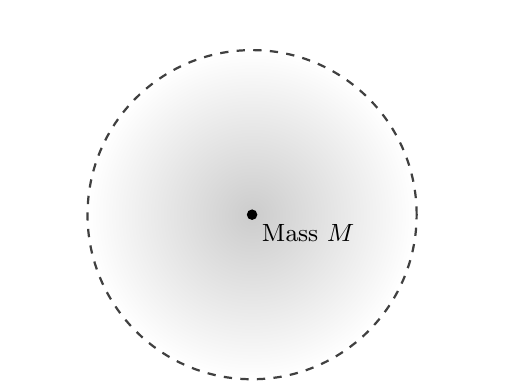
\begin{tikzpicture}[scale=0.95]
  % ----- Right Side: Gravitational Source Circle -----
  % Invisible bounding box matching the height of the left grid to maintain perfect baseline alignment
  \useasboundingbox (-3, 0) rectangle (3, 4.5);
  
  % Centered Gravitational Source (shifted vertically to center elegantly next to the grid)
  \begin{scope}[shift={(0, 2)}]
    \shade[inner color=gray!40, outer color=white] (0, 0) circle (2.2);
    \draw[thick, dashed, darkgray] (0, 0) circle (2.2);
    \fill (0, 0) circle (2pt) node[below right, font=\small] {Mass $M$};
  \end{scope}
\end{tikzpicture}
\end{minipage}
\caption{Geodesic deviation as a manifestation of spacetime curvature. In the presence of a central gravitating mass $M$ (right), freely falling test particles converge along radial trajectories. This tidal convergence (left) causes initially parallel worldlines to mutually accelerate, breaking the global validity of parallel transport.}
\label{fig:geodesic_deviation}
\end{figure}


\begin{figure}[htbp]
\centering
\begin{minipage}{0.48\textwidth}
\centering
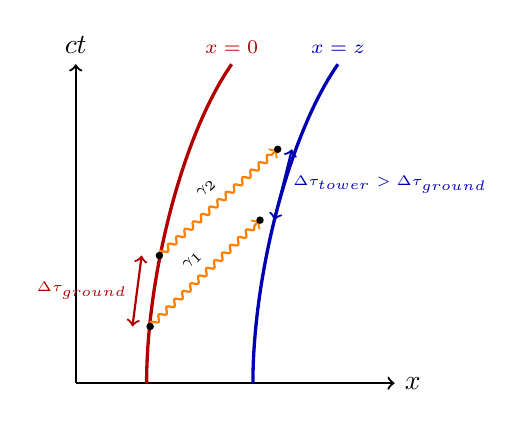
\begin{tikzpicture}[scale=0.9]
  % ----- Left Side: Spacetime Diagram -----
  % Axes
  \draw[->, thick] (0,0) -- (0, 4.5) node[above] {$ct$};
  \draw[->, thick] (0,0) -- (4.5, 0) node[right] {$x$};

  % Worldlines (Rindler-like curving)
  \draw[very thick, red!70!black] (1, 0) .. controls (1, 1.5) and (1.5, 3.5) .. (2.2, 4.5) 
    node[above, font=\scriptsize] {$x=0$};
  \draw[very thick, blue!70!black] (2.5, 0) .. controls (2.5, 1.5) and (3.0, 3.5) .. (3.7, 4.5) 
    node[above, font=\scriptsize] {$x=z$};

  % Photon 1
  \coordinate (E1) at (1.05, 0.8);
  \coordinate (R1) at (2.6, 2.3);
  \draw[->, thick, orange, decorate, decoration={snake, amplitude=1pt, segment length=4pt, post length=2pt}] 
    (E1) -- (R1) node[midway, sloped, above=1pt, text=black, font=\tiny] {$\gamma_1$};
  \fill (E1) circle (1.5pt); \fill (R1) circle (1.5pt);

  % Photon 2
  \coordinate (E2) at (1.18, 1.8);
  \coordinate (R2) at (2.85, 3.3);
  \draw[->, thick, orange, decorate, decoration={snake, amplitude=1pt, segment length=4pt, post length=2pt}] 
    (E2) -- (R2) node[midway, sloped, above=1pt, text=black, font=\tiny] {$\gamma_2$};
  \fill (E2) circle (1.5pt); \fill (R2) circle (1.5pt);

  % Time intervals
  \draw[<->, thick, red!70!black] (0.8, 0.8) -- (0.93, 1.8) 
    node[midway, left, font=\tiny] {$\Delta \tau_{\text{ground}}$};
  \draw[<->, thick, blue!70!black] (2.8, 2.3) -- (3.05, 3.3) 
    node[midway, right, font=\tiny] {$\Delta \tau_{\text{tower}} > \Delta \tau_{\text{ground}}$};
\end{tikzpicture}
\end{minipage}
\hfill
\begin{minipage}{0.48\textwidth}
\centering
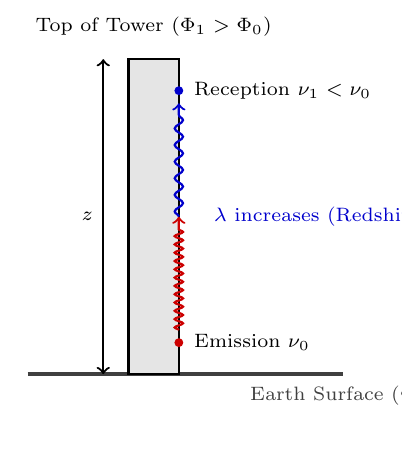
\begin{tikzpicture}[scale=0.8]
  % ----- Right Side: Physical Tower Diagram -----
  % Establish matching vertical bounds to ensure perfect alignment
  \useasboundingbox (-2, -0.8) rectangle (3.5, 5.5);

  % Ground Surface
  \draw[ultra thick, darkgray] (-2,0) -- (3,0) node[below, font=\scriptsize] {Earth Surface ($\Phi_0$)};
  
  % Tower
  \draw[thick, fill=gray!20] (-0.4, 0) rectangle (0.4, 5);
  \draw[<->, thick] (-0.8, 0) -- (-0.8, 5) node[midway, left, font=\scriptsize] {$z$};
  \node[above, font=\scriptsize] at (0, 5.2) {Top of Tower ($\Phi_1 > \Phi_0$)};

  % Photon Emission (Bottom)
  \fill[red!80!black] (0.4, 0.5) circle (2pt) node[right=2pt, text=black, font=\scriptsize] {Emission $\nu_0$};
  
  % Photon Reception (Top)
  \fill[blue!80!black] (0.4, 4.5) circle (2pt) node[right=2pt, text=black, font=\scriptsize] {Reception $\nu_1 < \nu_0$};

  % Wavelength stretch visualization
  \draw[->, thick, decorate, decoration={snake, amplitude=1.5pt, segment length=3pt, post length=4pt}, red!80!black] 
    (0.4, 0.7) -- (0.4, 2.5);
  \draw[->, thick, decorate, decoration={snake, amplitude=1.5pt, segment length=6pt, post length=4pt}, blue!80!black] 
    (0.4, 2.5) -- (0.4, 4.3);
    
  \node[right, font=\scriptsize, text=blue!80!black] at (0.8, 2.5) {$\lambda$ increases (Redshift)};
\end{tikzpicture}
\end{minipage}
\caption{Gravitational redshift and relative time dilation. The spacetime diagram (left) models the metric variation where the proper time interval $\Delta \tau_{\text{tower}}$ between successive photon wavecrests is strictly greater than $\Delta \tau_{\text{ground}}$. The physical schematic (right) models an experimental setup (e.g., Pound-Rebka) where an observer at a higher gravitational potential ($\Phi_1$) measures an increase in the emitted photon's wavelength.}
\label{fig:gravitational_redshift}
\end{figure}


\begin{figure}[htbp]
\centering
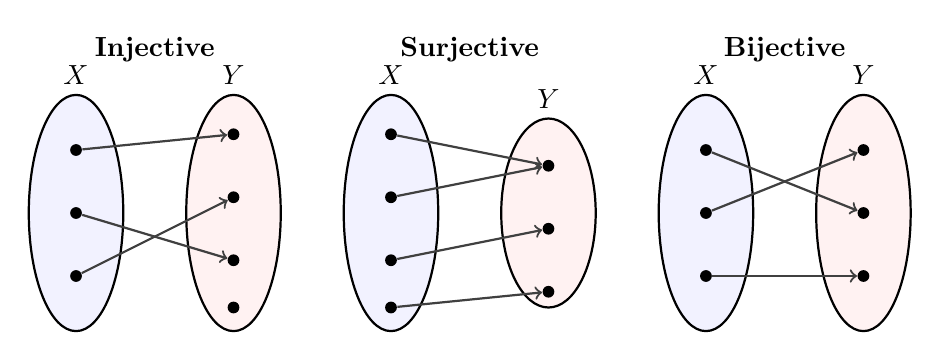
\begin{tikzpicture}[scale=1]
  \tikzset{dot/.style={circle, fill=black, inner sep=1.5pt}}
  
  % Injective
  \begin{scope}[shift={(0,0)}]
    \node[above, font=\bfseries] at (1, 2.8) {Injective};
    \draw[thick, fill=blue!5] (0, 1) ellipse (0.6 and 1.5) node[above=1.5cm] {$X$};
    \draw[thick, fill=red!5] (2, 1) ellipse (0.6 and 1.5) node[above=1.5cm] {$Y$};
    \node[dot] (a1) at (0, 1.8) {}; \node[dot] (a2) at (0, 1) {}; \node[dot] (a3) at (0, 0.2) {};
    \node[dot] (b1) at (2, 2) {}; \node[dot] (b2) at (2, 1.2) {}; \node[dot] (b3) at (2, 0.4) {}; \node[dot] (b4) at (2, -0.2) {};
    \draw[->, thick, darkgray] (a1) -- (b1); 
    \draw[->, thick, darkgray] (a2) -- (b3); 
    \draw[->, thick, darkgray] (a3) -- (b2);
  \end{scope}

  % Surjective
  \begin{scope}[shift={(4,0)}]
    \node[above, font=\bfseries] at (1, 2.8) {Surjective};
    \draw[thick, fill=blue!5] (0, 1) ellipse (0.6 and 1.5) node[above=1.5cm] {$X$};
    \draw[thick, fill=red!5] (2, 1) ellipse (0.6 and 1.2) node[above=1.2cm] {$Y$};
    \node[dot] (c1) at (0, 2) {}; \node[dot] (c2) at (0, 1.2) {}; \node[dot] (c3) at (0, 0.4) {}; \node[dot] (c4) at (0, -0.2) {};
    \node[dot] (d1) at (2, 1.6) {}; \node[dot] (d2) at (2, 0.8) {}; \node[dot] (d3) at (2, 0) {};
    \draw[->, thick, darkgray] (c1) -- (d1); 
    \draw[->, thick, darkgray] (c2) -- (d1); 
    \draw[->, thick, darkgray] (c3) -- (d2); 
    \draw[->, thick, darkgray] (c4) -- (d3);
  \end{scope}

  % Bijective
  \begin{scope}[shift={(8,0)}]
    \node[above, font=\bfseries] at (1, 2.8) {Bijective};
    \draw[thick, fill=blue!5] (0, 1) ellipse (0.6 and 1.5) node[above=1.5cm] {$X$};
    \draw[thick, fill=red!5] (2, 1) ellipse (0.6 and 1.5) node[above=1.5cm] {$Y$};
    \node[dot] (e1) at (0, 1.8) {}; \node[dot] (e2) at (0, 1) {}; \node[dot] (e3) at (0, 0.2) {};
    \node[dot] (f1) at (2, 1.8) {}; \node[dot] (f2) at (2, 1) {}; \node[dot] (f3) at (2, 0.2) {};
    \draw[->, thick, darkgray] (e1) -- (f2); 
    \draw[->, thick, darkgray] (e2) -- (f1); 
    \draw[->, thick, darkgray] (e3) -- (f3);
  \end{scope}
\end{tikzpicture}
\caption{Classification of fundamental mappings between sets $X$ and $Y$. An injective function maps distinct elements to distinct outputs; a surjective function fully covers the codomain; and a bijective function satisfies both properties, establishing a rigorous one-to-one correspondence.}
\label{fig:mapping_types}
\end{figure}


\begin{figure}[htbp]
\centering
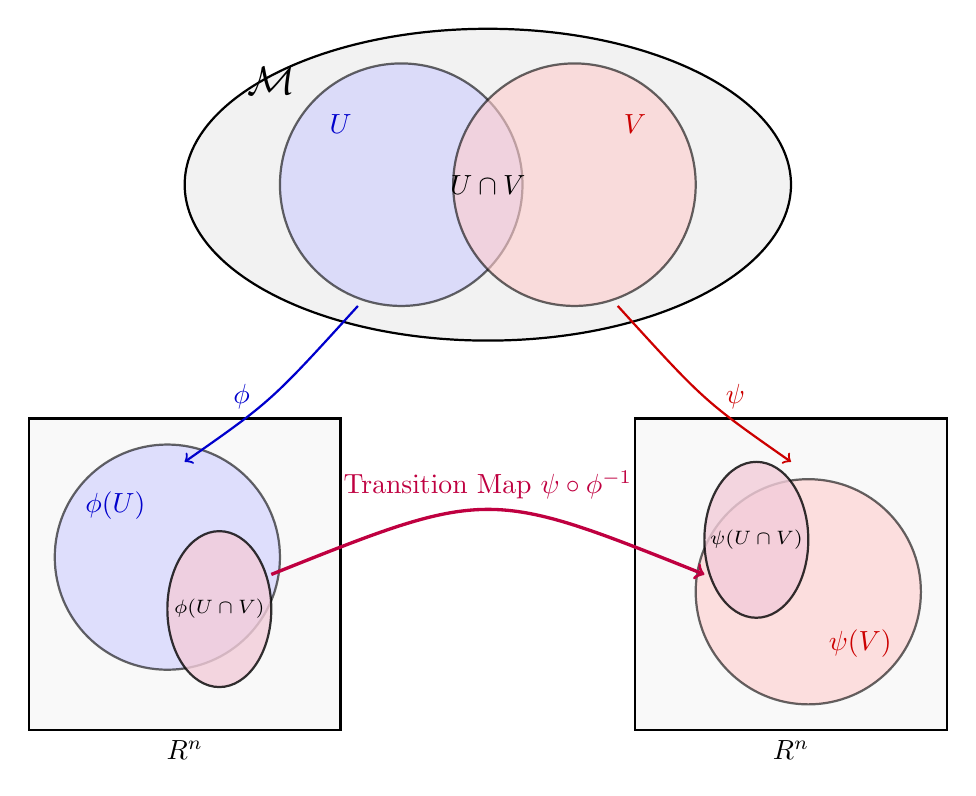
\begin{tikzpicture}[scale=1.1]
  % Manifold M
  \draw[thick, fill=gray!10] (0,0) ellipse (3.5 and 1.8);
  \node[font=\Large\bfseries] at (-2.5, 1.2) {$\mathcal{M}$};
  
  % Sets U and V
  \draw[thick, fill=blue!20, opacity=0.6] (-1, 0) circle (1.4);
  \node[blue!80!black, font=\bfseries] at (-1.7, 0.7) {$U$};
  
  \draw[thick, fill=red!20, opacity=0.6] (1, 0) circle (1.4);
  \node[red!80!black, font=\bfseries] at (1.7, 0.7) {$V$};
  
  % U intersect V (Manifold)
  \node[font=\bfseries] at (0, 0) {$U \cap V$};
  
  % Chart 1 (Left) - R^n space
  \begin{scope}[shift={(-3.5, -4.5)}]
    \draw[thick, fill=gray!5] (-1.8, -1.8) rectangle (1.8, 1.8);
    \node[below] at (0, -1.8) {$\mathbb{R}^n$};
    \draw[thick, fill=blue!20, opacity=0.6] (-0.2,0.2) circle (1.3);
    \node[blue!80!black] at (-0.8, 0.8) {$\phi(U)$};
    % Image of intersection
    \draw[thick, fill=purple!20, opacity=0.8] (0.4,-0.4) ellipse (0.6 and 0.9);
    \node[font=\scriptsize, align=center] at (0.4, -0.4) {$\phi(U \cap V)$};
  \end{scope}

  % Chart 2 (Right) - R^n space
  \begin{scope}[shift={(3.5, -4.5)}]
    \draw[thick, fill=gray!5] (-1.8, -1.8) rectangle (1.8, 1.8);
    \node[below] at (0, -1.8) {$\mathbb{R}^n$};
    \draw[thick, fill=red!20, opacity=0.6] (0.2,-0.2) circle (1.3);
    \node[red!80!black] at (0.8, -0.8) {$\psi(V)$};
    % Image of intersection
    \draw[thick, fill=purple!20, opacity=0.8] (-0.4,0.4) ellipse (0.6 and 0.9);
    \node[font=\scriptsize, align=center] at (-0.4, 0.4) {$\psi(U \cap V)$};
  \end{scope}
  
  % Mappings from Manifold to R^n
  \draw[->, thick, blue!80!black] (-1.5, -1.4) .. controls (-2.5, -2.5) .. (-3.5, -3.2) node[midway, left=4pt] {$\phi$};
  \draw[->, thick, red!80!black] (1.5, -1.4) .. controls (2.5, -2.5) .. (3.5, -3.2) node[midway, right=4pt] {$\psi$};
  
  % Transition Map between R^n charts
  \draw[->, very thick, purple] (-2.5, -4.5) .. controls (0, -3.5) .. (2.5, -4.5) node[midway, above] {Transition Map $\psi \circ \phi^{-1}$};
\end{tikzpicture}
\caption{The foundational atlas construction of a differentiable manifold $\mathcal{M}$. Open subsets $U$ and $V$ are mapped to Euclidean space $\mathbb{R}^n$ via the local coordinate charts $\phi$ and $\psi$. The compatibility of these charts is guaranteed by the smoothness of the transition map $\psi \circ \phi^{-1}$ operating within the image of the overlap region $U \cap V$.}
\label{fig:transition_map}
\end{figure}


\begin{figure}[htbp]
\centering
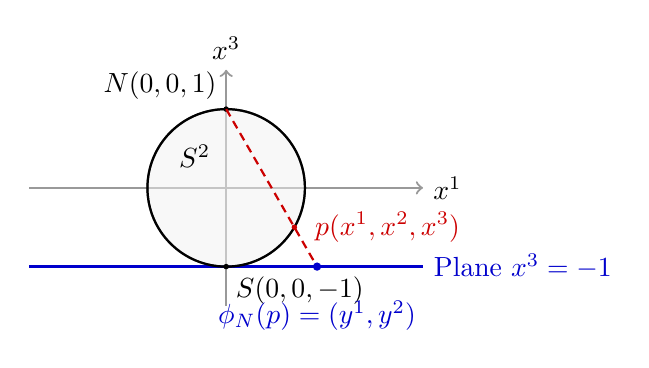
\begin{tikzpicture}[scale=1.0]
  % Axes
  \draw[->, thick, gray!80] (-2.5, 0) -- (2.5, 0) node[right, text=black] {$x^1$};
  \draw[->, thick, gray!80] (0, -1.5) -- (0, 1.5) node[above, text=black] {$x^3$};

  % Projection Plane x^3 = -1
  \draw[very thick, blue!80!black] (-2.5, -1) -- (2.5, -1) node[right] {Plane $x^3 = -1$};

  % Sphere S^2 cross-section (S^1)
  \draw[thick, fill=gray!10, opacity=0.5] (0,0) circle (1);
  \draw[thick] (0,0) circle (1);
  \node at (-0.4, 0.4) {$S^2$};
  
  % Poles
  \fill[black] (0, 1) circle (1pt) node[above left] {$N (0,0,1)$};
  \fill[black] (0, -1) circle (1pt) node[below right] {$S (0,0,-1)$};

  % Point P on the sphere (picking an arbitrary point)
  \coordinate (P) at (0.866, -0.5); % (sin(60), -cos(60))
  \fill[red!80!black] (P) circle (1pt) node[right=4pt] {$p (x^1, x^2, x^3)$};

  % Projection line from N through P to the plane
  % The line intersects z=-1 at x = 2/sqrt(3) ≈ 1.154
  \coordinate (Proj) at (1.154, -1);
  \draw[thick, densely dashed, red!80!black] (0,1) -- (Proj);
  
  % Projected point on the plane
  \fill[blue!80!black] (Proj) circle (1.5pt) node[below=9pt] {$\phi_N(p) = (y^1, y^2)$};
\end{tikzpicture}
\caption{Stereographic projection of the 2-sphere ($S^2$) from the North pole $N$ onto the tangent plane at the South pole ($x^3 = -1$). This geometric mapping provides a smooth, global coordinate chart covering the entire sphere excluding the projection pole itself ($S^2 \setminus \{N\}$).}
\label{fig:stereographic_projection}
\end{figure}

% Drawing 1: Composition of mappings between spaces (Manifolds)
\begin{figure}[htbp]
\centering
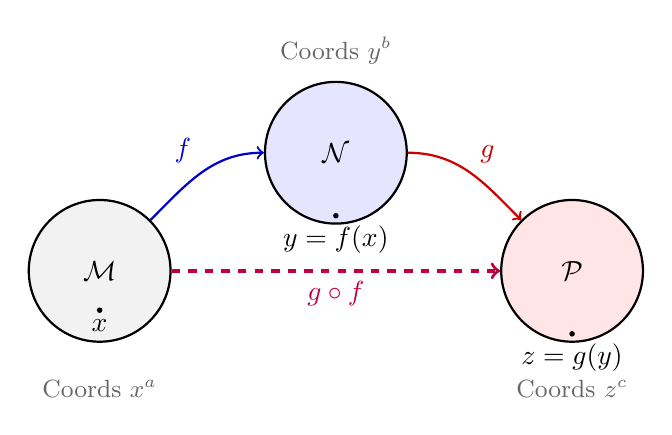
\begin{tikzpicture}[scale=1.0]
  % Spaces
  \node (M) at (0,0) [circle, draw, thick, fill=gray!10, minimum size=1.8cm] {$\mathcal{M}$};
  \node (N) at (3,1.5) [circle, draw, thick, fill=blue!10, minimum size=1.8cm] {$\mathcal{N}$};
  \node (P) at (6,0) [circle, draw, thick, fill=red!10, minimum size=1.8cm] {$\mathcal{P}$};

  % Mappings
  \draw[->, thick, blue!80!black] (M) to[out=45, in=180] node[midway, above left] {$f$} (N);
  \draw[->, thick, red!80!black] (N) to[out=0, in=135] node[midway, above right] {$g$} (P);
  \draw[->, very thick, dashed, purple] (M) to[out=0, in=180] node[midway, below] {$g \circ f$} (P);
  
  % Points and Coordinates
  \fill[black] (0.0, -0.5) circle (1pt) node[below] {$x$};
  \fill[black] (3, 0.7) circle (1pt) node[below] {$y = f(x)$};
  \fill[black] (6.0, -0.8) circle (1pt) node[below] {$z = g(y)$};
  
  % Coordinate system labels
  \node[font=\small, text=gray!80!black] at (0, -1.5) {Coords $x^a$};
  \node[font=\small, text=gray!80!black] at (3, 2.8) {Coords $y^b$};
  \node[font=\small, text=gray!80!black] at (6, -1.5) {Coords $z^c$};
\end{tikzpicture}
\caption{Composition of smooth maps between manifolds.}
\label{fig:map_composition}
\end{figure}


% Drawing 2: Curved surface with coordinate lines and tangent basis
\begin{figure}[htbp]
\centering
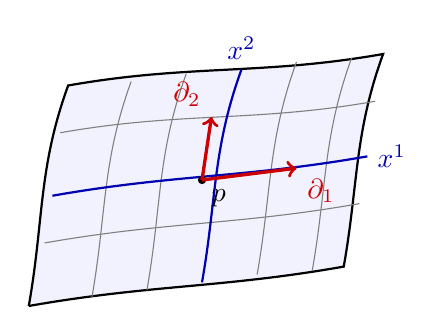
\begin{tikzpicture}[scale=1.0]
  % Define point p
  \coordinate (P) at (2.2, 1.6);

  % Curved surface
  \draw[thick, fill=blue!5] (0,0) to[out=10, in=190] (4,0.5) 
        to[out=80, in=250] (4.5,3.2) 
        to[out=190, in=10] (0.5,2.8) 
        to[out=250, in=80] (0,0);
        
  % Coordinate lines (thin gray)
  \draw[gray, thin] (0.8, 0.1) to[out=80, in=250] (1.3, 2.85);
  \draw[gray, thin] (1.5, 0.2) to[out=80, in=250] (2.0, 2.95);
  \draw[gray, thin] (2.9, 0.4) to[out=80, in=250] (3.4, 3.1);
  \draw[gray, thin] (3.6, 0.45) to[out=80, in=250] (4.1, 3.15);

  \draw[gray, thin] (0.2, 0.8) to[out=10, in=190] (4.2, 1.3);
  \draw[gray, thin] (0.4, 2.2) to[out=10, in=190] (4.4, 2.6);

  % Highlighted coordinate lines passing through p
  % x^1 curve
  \draw[blue!70!black, thick] (0.3, 1.4) to[out=10, in=190] (4.3, 1.9) node[right] {$x^1$};
  % x^2 curve
  \draw[blue!70!black, thick] (2.2, 0.3) to[out=80, in=250] (2.7, 3.0) node[above] {$x^2$};

  % Mark point p
  \fill[black] (P) circle (1.5pt) node[below right] {$p$};

  % Tangent basis vectors
  \draw[->, very thick, red!80!black] (P) -- ++(1.2, 0.15) node[below right] {$\partial_1$};
  \draw[->, very thick, red!80!black] (P) -- ++(0.12, 0.8) node[above left] {$\partial_2$};

\end{tikzpicture}
\caption{Coordinate curves and their tangent basis vectors at a point $p$.}
\label{fig:tangent_basis}
\end{figure}


% Drawing 3: Curved surface patch with two overlapping coordinate grids
\begin{figure}[htbp]
\centering
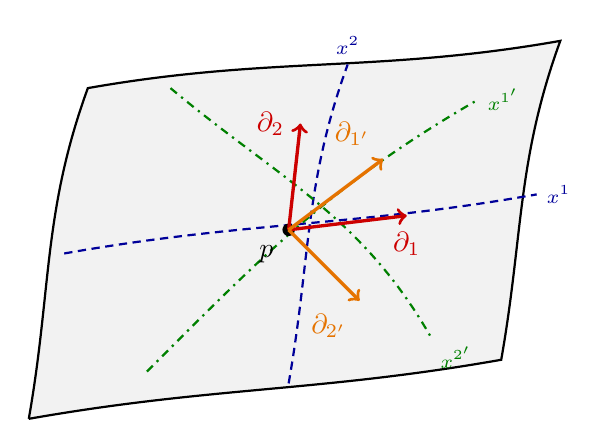
\begin{tikzpicture}[scale=1.5]
  % Define point p
  \coordinate (P) at (2.2, 1.6);

  % Curved surface patch
  \draw[thick, fill=gray!10] (0,0) to[out=10, in=190] (4,0.5) 
        to[out=80, in=250] (4.5,3.2) 
        to[out=190, in=10] (0.5,2.8) 
        to[out=250, in=80] (0,0);

  % Grid 1 (x^\mu) lines
  \draw[blue!60!black, thick, densely dashed] (0.3, 1.4) to[out=10, in=190] (4.3, 1.9) node[right, font=\scriptsize] {$x^1$};
  \draw[blue!60!black, thick, densely dashed] (2.2, 0.3) to[out=80, in=250] (2.7, 3.0) node[above, font=\scriptsize] {$x^2$};

  % Grid 2 (x^{\mu'}) lines
  \draw[green!50!black, thick, dash dot] (1.0, 0.4) to[out=45, in=210] (3.8, 2.7) node[right, font=\scriptsize] {$x^{1'}$};
  \draw[green!50!black, thick, dash dot] (1.2, 2.8) to[out=-40, in=120] (3.4, 0.7) node[below right, font=\scriptsize] {$x^{2'}$};

  % Mark point p
  \fill[black] (P) circle (1.5pt) node[below left=2pt] {$p$};

  % Basis Vectors for Grid 1 (Red)
  \draw[->, very thick, red!80!black] (P) -- ++(1.0, 0.12) node[below=2pt] {$\partial_1$};
  \draw[->, very thick, red!80!black] (P) -- ++(0.1, 0.9) node[left=2pt] {$\partial_2$};

  % Basis Vectors for Grid 2 (Orange)
  \draw[->, very thick, orange!90!black] (P) -- ++(0.8, 0.6) node[above left=1pt] {$\partial_{1'}$};
  \draw[->, very thick, orange!90!black] (P) -- ++(0.6, -0.6) node[below left=1pt] {$\partial_{2'}$};

\end{tikzpicture}
\caption{Transformation of basis vectors under a local coordinate change.}
\label{fig:coordinate_transformation}
\end{figure}


% Drawing 4: Infinitesimal triangle on a 2-sphere patch
\begin{figure}[htbp]
\centering
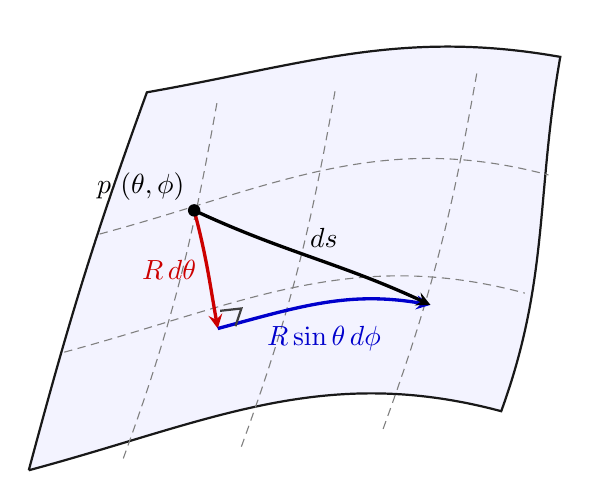
\begin{tikzpicture}[scale=1.5]
  % Draw a curved patch of the 2-sphere
  \draw[thick, fill=blue!5, opacity=0.9] (0,0) to[out=15, in=165] (4,0.5) 
        to[out=70, in=260] (4.5, 3.5) 
        to[out=170, in=10] (1, 3.2) 
        to[out=250, in=75] (0,0);
        
  % Grid lines (Lines of constant theta and phi) to imply curvature
  \draw[gray, thin, densely dashed] (0.8, 0.1) to[out=70, in=260] (1.6, 3.15);
  \draw[gray, thin, densely dashed] (1.8, 0.2) to[out=70, in=260] (2.6, 3.25);
  \draw[gray, thin, densely dashed] (3.0, 0.35) to[out=70, in=260] (3.8, 3.4);
  
  \draw[gray, thin, densely dashed] (0.3, 1.0) to[out=15, in=165] (4.2, 1.5);
  \draw[gray, thin, densely dashed] (0.6, 2.0) to[out=15, in=165] (4.4, 2.5);

  % Infinitesimal right-triangle points
  % A = Point p (theta, phi)
  % B = Point displaced by d\theta (theta + d\theta, phi)
  % C = Point displaced by d\theta and d\phi (theta + d\theta, phi + d\phi)
  \coordinate (A) at (1.4, 2.2);
  \coordinate (B) at (1.6, 1.2);
  \coordinate (C) at (3.4, 1.4);

  % d(theta) side (meridian - arc length R d\theta)
  \draw[very thick, red!80!black, -stealth] (A) to[out=285, in=100] (B);
  \node[left, red!80!black] at (1.5, 1.7) {$R \, d\theta$};

  % d(phi) side (parallel of latitude - arc length R \sin\theta d\phi)
  \draw[very thick, blue!80!black, -stealth] (B) to[out=15, in=170] (C);
  \node[below, blue!80!black] at (2.5, 1.3) {$R \sin\theta \, d\phi$};

  % ds side (hypotenuse - invariant interval)
  \draw[very thick, black, -stealth] (A) to[out=-25, in=155] (C);
  \node[above right, font=\bfseries] at (2.3, 1.8) {$ds$};

  % Mark the starting point
  \fill (A) circle (1.5pt) node[above left] {$p \ (\theta, \phi)$};

  % Fake right angle symbol (approximated for curved perspective)
  \draw[thick, darkgray] (1.75, 1.22) -- (1.8, 1.37) -- (1.62, 1.35);

\end{tikzpicture}
\caption{Infinitesimal line element $ds$ on the surface of a 2-sphere.}
\label{fig:sphere_line_element}
\end{figure}


% Drawing 5: Big Bang singularity and cosmological particle horizon
\begin{figure}[htbp]
\centering
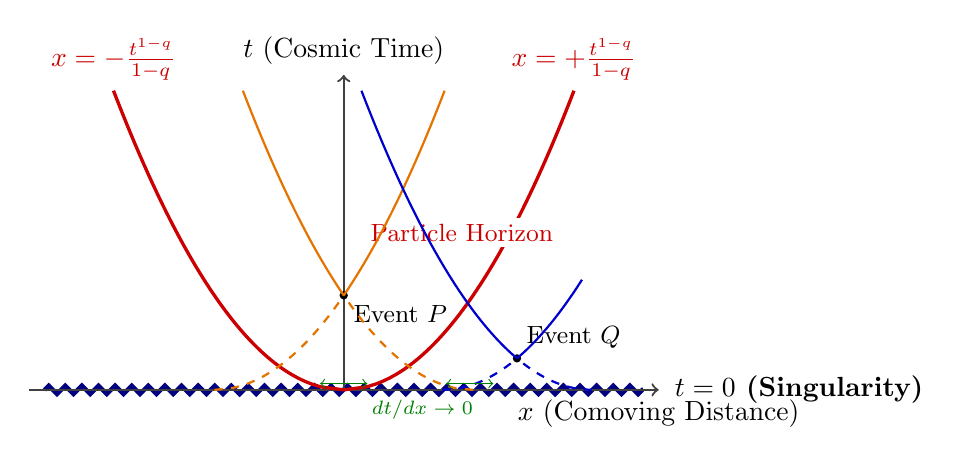
\begin{tikzpicture}[scale=1.0]
  % Singularity (Big Bang)
  \draw[ultra thick, decorate, decoration={zigzag, segment length=6pt, amplitude=1.5pt}, blue!50!black] 
    (-3.8, 0) -- (3.8, 0);
  \node[right=8pt, text=black, font=\bfseries] at (3.8, 0) {$t=0$ (Singularity)};

  % Axes
  \draw[->, thick, darkgray] (0, 0) -- (0, 4) node[above, text=black] {$t$ (Cosmic Time)};
  \draw[->, thick, darkgray] (-4, 0) -- (4, 0) node[below, text=black] {$x$ (Comoving Distance)};

  % Particle Horizon (Future light cone from origin)
  % Using a scale factor 1.5 for the x-coordinate to represent 1/(1-q)
  \draw[very thick, red!80!black, variable=\t, domain=0:3.8, samples=100] 
    plot ({1.5*sqrt(\t)}, {\t}) node[above] {$x = +\frac{t^{1-q}}{1-q}$};
  \draw[very thick, red!80!black, variable=\t, domain=0:3.8, samples=100] 
    plot ({-1.5*sqrt(\t)}, {\t}) node[above] {$x = -\frac{t^{1-q}}{1-q}$};
  \node[red!80!black, fill=white, inner sep=2pt, font=\small] at (1.5, 2.0) {Particle Horizon};

  % Event P and its light cone
  \fill (0, 1.2) circle (1.5pt) node[below right, font=\small] {Event $P$};
  
  % Future light cone of P
  \draw[thick, orange!90!black, variable=\t, domain=1.2:3.8, samples=100] 
    plot ({1.5*(sqrt(\t) - sqrt(1.2))}, {\t});
  \draw[thick, orange!90!black, variable=\t, domain=1.2:3.8, samples=100] 
    plot ({-1.5*(sqrt(\t) - sqrt(1.2))}, {\t});
    
  % Past light cone of P (arriving rays)
  \draw[thick, dashed, orange!90!black, variable=\t, domain=0:1.2, samples=50] 
    plot ({1.5*(sqrt(\t) - sqrt(1.2))}, {\t});
  \draw[thick, dashed, orange!90!black, variable=\t, domain=0:1.2, samples=50] 
    plot ({-1.5*(sqrt(\t) - sqrt(1.2))}, {\t});

  % Event Q and its light cone (off-center)
  \fill (2.2, 0.4) circle (1.5pt) node[above right, font=\small] {Event $Q$};
  
  % Future light cone of Q (bounded to graph limits)
  \draw[thick, blue!80!black, variable=\t, domain=0.4:1.4, samples=100] 
    plot ({2.2 + 1.5*(sqrt(\t) - sqrt(0.4))}, {\t});
  \draw[thick, blue!80!black, variable=\t, domain=0.4:3.8, samples=100] 
    plot ({2.2 - 1.5*(sqrt(\t) - sqrt(0.4))}, {\t});
    
  % Past light cone of Q
  \draw[thick, dashed, blue!80!black, variable=\t, domain=0:0.4, samples=50] 
    plot ({2.2 + 1.5*(sqrt(\t) - sqrt(0.4))}, {\t});
  \draw[thick, dashed, blue!80!black, variable=\t, domain=0:0.4, samples=50] 
    plot ({2.2 - 1.5*(sqrt(\t) - sqrt(0.4))}, {\t});

  % Annotations highlighting tangent behavior at t=0
  \draw[<->, green!50!black, thin] (1.3, 0.08) -- (1.9, 0.08);
  \node[green!50!black, below, font=\scriptsize] at (1, 0) {$dt/dx \to 0$};
  
  \draw[<->, green!50!black, thin] (-0.3, 0.08) -- (0.3, 0.08);

\end{tikzpicture}
\caption{Spacetime diagram illustrating the cosmological particle horizon.}
\label{fig:particle_horizon}
\end{figure}


% Drawing 6: Spacelike Surface S with its Domains of Dependence
\begin{figure}[htbp]
\centering
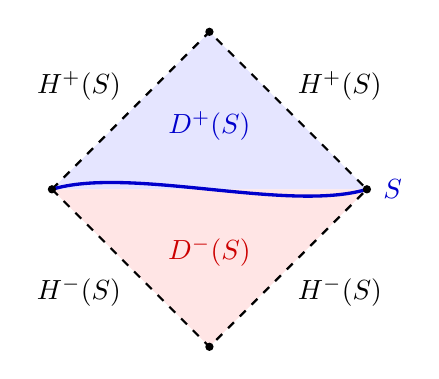
\begin{tikzpicture}[scale=1]
  % D+(S) Region
  \draw[thick, fill=blue!10, dashed] (-2,0) -- (0, 2) -- (2,0);
  % D-(S) Region
  \draw[thick, fill=red!10, dashed] (-2,0) -- (0, -2) -- (2,0);
  
  % Spacelike Surface S
  \draw[very thick, blue!80!black] (-2,0) .. controls (-1, 0.3) and (1, -0.3) .. (2,0) node[right=2pt] {$S$};
  
  % Labels
  \node[blue!80!black, font=\bfseries] at (0, 0.8) {$D^+(S)$};
  \node[red!80!black, font=\bfseries] at (0, -0.8) {$D^-(S)$};
  
  \node[above left] at (-1, 1) {$H^+(S)$};
  \node[above right] at (1, 1) {$H^+(S)$};
  
  \node[below left] at (-1, -1) {$H^-(S)$};
  \node[below right] at (1, -1) {$H^-(S)$};

  \fill (0,2) circle (1.5pt);
  \fill (0,-2) circle (1.5pt);
  \fill (-2,0) circle (1.5pt);
  \fill (2,0) circle (1.5pt);
\end{tikzpicture}
\caption{Domains of dependence and Cauchy horizons for a spacelike surface $S$.}
\label{fig:domain_of_dependence}
\end{figure}


% Drawing 7: Past light cone intersecting an incomplete hypersurface S
\begin{figure}[htbp]
\centering
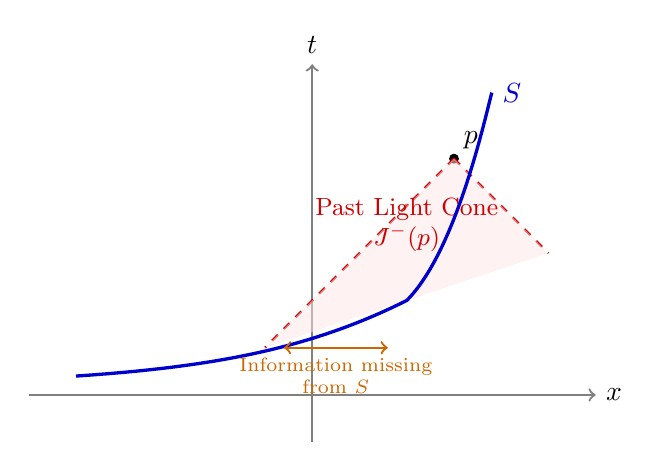
\begin{tikzpicture}[scale=1.2]
  % Axes
  \draw[->, thick, gray] (0,-0.5) -- (0, 3.5) node[above, text=black] {$t$};
  \draw[->, thick, gray] (-3,0) -- (3, 0) node[right, text=black] {$x$};
  
  % Point p
  \coordinate (P) at (1.5, 2.5);
  \fill[black] (P) circle (1.5pt) node[above right] {$p$};
  
  % Past Light Cone of p
  \draw[thick, red!80!black, dashed] (P) -- (-0.5, 0.5);
  \draw[thick, red!80!black, dashed] (P) -- (2.5, 1.5);
  \fill[red!10, opacity=0.5] (P) -- (-0.5, 0.5) -- (2.5, 1.5) -- cycle;
  \node[red!80!black, font=\small, align=center] at (1.0, 1.8) {Past Light Cone\\$J^-(p)$};

  % Hypersurface S (asymptotically approaching a null line, bounded)
  \draw[very thick, blue!80!black] (-2.5, 0.2) .. controls (-1, 0.3) and (0, 0.5) .. (1, 1) .. controls (1.5, 1.5) and (1.8, 2.8) .. (1.9, 3.2) node[right] {$S$};
  
  % Highlight intersection failure
  \draw[<->, thick, orange!80!black] (-0.3, 0.5) -- (0.8, 0.5) node[midway, below, font=\scriptsize, align=center] {Information missing\\from $S$};
\end{tikzpicture}
\caption{An incomplete Cauchy surface $S$ failing to capture the full past of $p$.}
\label{fig:incomplete_cauchy}
\end{figure}


% Drawing 8: Tipping light cones and Closed Timelike Curve (CTC)
\begin{figure}[htbp]
\centering
\begin{tikzpicture}[scale=1]
  % Cylinder background (back half)
  \draw[thick, dashed, gray] (1.5, 2.5) arc (0:180:1.5 and 0.4);
  \draw[thick, dashed, gray] (1.5, -2.5) arc (0:180:1.5 and 0.4);
  
  % Cylinder fill
  \path[fill=gray!5] (-1.5,-2.5) -- (-1.5,2.5) arc (180:360:1.5 and 0.4) -- (1.5,-2.5) arc (360:180:1.5 and 0.4) -- cycle;
  
  % Cylinder foreground
  \draw[thick] (-1.5, -2.5) -- (-1.5, 2.5);
  \draw[thick] (1.5, -2.5) -- (1.5, 2.5);
  \draw[thick] (-1.5, 2.5) arc (180:360:1.5 and 0.4);
  \draw[thick] (-1.5, -2.5) arc (180:360:1.5 and 0.4);

  % Axis
  \draw[->, thick, gray, dashed] (0, -3) -- (0, 3) node[above, text=black] {$t$};

  % Upright Light Cone (Bottom)
  \begin{scope}[shift={(0, -1.8)}]
    \fill[red!20, opacity=0.8] (0,0) -- (-0.3, 0.5) arc (180:360:0.3 and 0.08) -- cycle;
    \draw[thick, red!80!black] (0,0) -- (-0.3, 0.5);
    \draw[thick, red!80!black] (0,0) -- (0.3, 0.5);
    \draw[thick, red!80!black] (-0.3, 0.5) arc (180:360:0.3 and 0.08);
    \draw[thick, red!80!black, dashed] (0.3, 0.5) arc (0:180:0.3 and 0.08);
    \fill (0,0) circle (1pt);
  \end{scope}

  % Tilted Light Cone (Middle)
  \begin{scope}[shift={(0, -0.2)}]
    \fill[red!20, opacity=0.8] (0,0) -- (0.1, 0.5) arc (150:330:0.25 and 0.1) -- cycle;
    \draw[thick, red!80!black] (0,0) -- (0.1, 0.5);
    \draw[thick, red!80!black] (0,0) -- (0.5, 0.26);
    \draw[thick, red!80!black] (0.1, 0.5) arc (150:330:0.25 and 0.1);
    \draw[thick, red!80!black, dashed] (0.5, 0.26) arc (-30:150:0.25 and 0.1);
    \fill (0,0) circle (1pt);
  \end{scope}

  % Tipped Light Cone (Top - tangent to CTC)
  \begin{scope}[shift={(0, 1.5)}]
    \fill[red!20, opacity=0.8] (0,0) -- (0.5, 0.15) arc (60:240:0.08 and 0.2) -- cycle;
    \draw[thick, red!80!black] (0,0) -- (0.5, 0.15);
    \draw[thick, red!80!black] (0,0) -- (0.5, -0.25);
    \draw[thick, red!80!black] (0.5, -0.25) arc (240:420:0.08 and 0.2);
    \fill (0,0) circle (1pt);
  \end{scope}

  % Closed Timelike Curve (CTC) at t = 1.5
  \draw[very thick, blue!80!black, decoration={markings, mark=at position 0.3 with {\arrow{>}}, mark=at position 0.8 with {\arrow{>}}}, postaction={decorate}] (0, 1.5) ellipse (1.5 and 0.4);
  \node[blue!80!black, right] at (1.5, 1.5) {CTC};

\end{tikzpicture}
\caption{Tipping of light cones leading to the formation of a Closed Timelike Curve.}
\label{fig:ctc_cylinder}
\end{figure}


% Drawing 9: Singularity and Unpredictable Region beyond Cauchy Horizon
\begin{figure}[htbp]
\centering
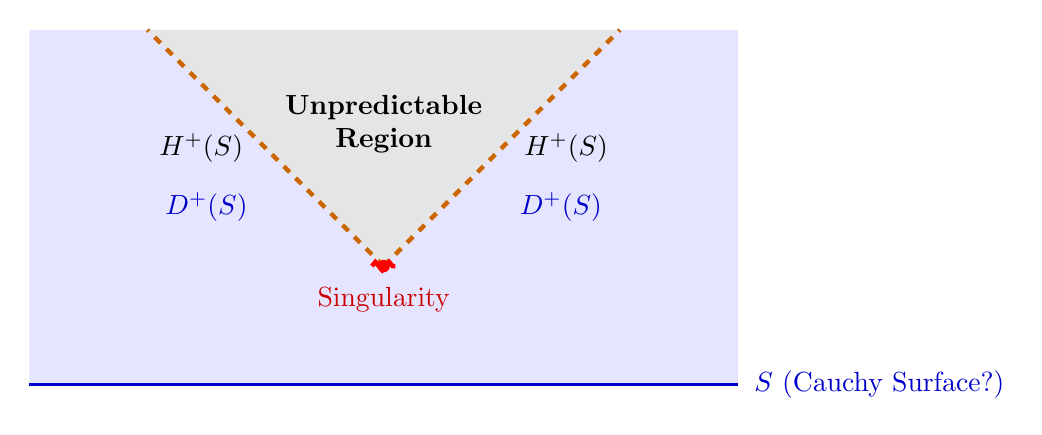
\begin{tikzpicture}[scale=1.5]
  % Future Light Cone of the Singularity (Unpredictable Region)
  \fill[gray!20] (0, 1) -- (-2, 3) -- (2, 3) -- cycle;
  
  % Domain of Dependence D+(S)
  \fill[blue!10] (-3, 0) -- (-3, 3) -- (-2, 3) -- (0, 1) -- (2, 3) -- (3, 3) -- (3, 0) -- cycle;

  % Cauchy Horizon H+(S)
  \draw[ultra thick, dashed, orange!80!black] (0, 1) -- (-2, 3) node[midway, left=4pt, text=black] {$H^+(S)$};
  \draw[ultra thick, dashed, orange!80!black] (0, 1) -- (2, 3) node[midway, right=4pt, text=black] {$H^+(S)$};

  % Singularity
  \draw[ultra thick, decorate, decoration={zigzag, segment length=5pt, amplitude=1.5pt}, red] (-0.1, 1) -- (0.1, 1);
  \fill[red] (0,1) circle (1.5pt);
  \node[red!80!black, below] at (0, 0.9) {Singularity};

  % Spacelike Surface S
  \draw[very thick, blue!80!black] (-3, 0) -- (3, 0) node[right=2pt] {$S$ (Cauchy Surface?)};

  % Labels
  \node[blue!80!black, font=\bfseries] at (-1.5, 1.5) {$D^+(S)$};
  \node[blue!80!black, font=\bfseries] at (1.5, 1.5) {$D^+(S)$};
  
  \node[font=\bfseries, align=center] at (0, 2.2) {Unpredictable\\Region};
  
\end{tikzpicture}
\caption{Breakdown of predictability beyond the Cauchy horizon due to a singularity.}
\label{fig:cauchy_horizon_singularity}
\end{figure}


% Drawing 1: 3D Volume Element / Basis Vectors
\begin{figure}[htbp]
\centering
\begin{tikzpicture}[scale=1.2, line join=round, line cap=round]
  % Define origin and basis vectors
  \coordinate (O) at (0,0);
  \coordinate (V1) at (2.5, -0.4);
  \coordinate (V2) at (1.2, 1.2);
  \coordinate (V3) at (0, 2.2);

  % Calculate vertices
  \coordinate (V12) at ($(V1)+(V2)$);
  \coordinate (V13) at ($(V1)+(V3)$);
  \coordinate (V23) at ($(V2)+(V3)$);
  \coordinate (V123) at ($(V1)+(V2)+(V3)$);

  % Draw hidden (back) edges
  \draw[thick, dashed, gray] (O) -- (V2);
  \draw[thick, dashed, gray] (V2) -- (V12);
  \draw[thick, dashed, gray] (V2) -- (V23);

  % Fill visible faces with varying opacity for 3D effect
  \fill[gray!20, opacity=0.85] (O) -- (V1) -- (V13) -- (V3) -- cycle; % Front
  \fill[gray!40, opacity=0.85] (V1) -- (V12) -- (V123) -- (V13) -- cycle; % Right
  \fill[gray!10, opacity=0.85] (V3) -- (V13) -- (V123) -- (V23) -- cycle; % Top

  % Draw visible edges
  \draw[thick] (O) -- (V1) -- (V12) -- (V123) -- (V23) -- (V3) -- cycle;
  \draw[thick] (V1) -- (V13) -- (V3);
  \draw[thick] (V13) -- (V123);

  % Draw the three primary vectors
  \draw[->, very thick, red!80!black] (O) -- (V1) node[midway, below=2pt] {$dx^{(1)}$};
  \draw[->, very thick, green!60!black] (O) -- (V2) node[midway, below right] {$dx^{(2)}$};
  \draw[->, very thick, blue!80!black] (O) -- (V3) node[midway, left=2pt] {$dx^{(3)}$};

  % Label the volume
\node[font=\bfseries, align=center] at (1.9, 2.5) {Volume element \\ $\epsilon = \sqrt{|g|} d^n x$};
\end{tikzpicture}
\caption{The invariant volume element in a curved space.}
\label{fig:volume_element}
\end{figure}


% Drawing 2: Parallel Transport on a Sphere
\begin{figure}[htbp]
\centering
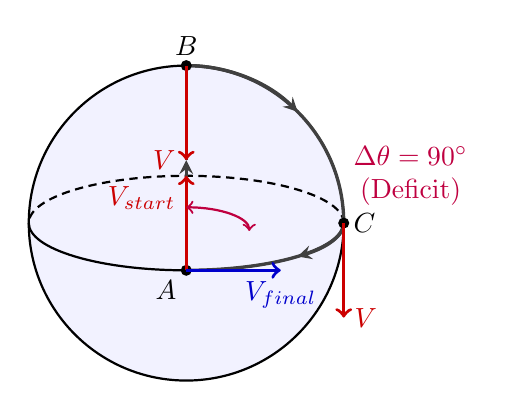
\begin{tikzpicture}[scale=2]
  % Sphere Base
  \draw[thick, fill=blue!5] (0,0) circle (1);
  
  % Equator
  \draw[thick, densely dashed] (1,0) arc (0:180:1 and 0.3);
  \draw[thick] (-1,0) arc (180:360:1 and 0.3);

  % Geodesic Paths
  % Path A -> B (Central Meridian)
  \draw[very thick, darkgray, -stealth] (0,-0.3) -- (0, 0.4);
  \draw[very thick, darkgray] (0,0.4) -- (0,1);
  
  % Path B -> C (Right Meridian)
  \draw[very thick, darkgray, -stealth] (0,1) arc (90:45:1 and 1);
  \draw[very thick, darkgray] (0,1) arc (90:0:1 and 1);
  
  % Path C -> A (Equator segment)
  \draw[very thick, darkgray, -stealth] (1,0) arc (360:315:1 and 0.3);
  \draw[very thick, darkgray] (1,0) arc (360:270:1 and 0.3);

  % Key Points
  \fill (0,-0.3) circle (1pt) node[below left] {$A$};
  \fill (0,1) circle (1pt) node[above] {$B$};
  \fill (1,0) circle (1pt) node[right] {$C$};

  % Transported Vectors
  % Initial Vector at A (Pointing North)
  \draw[->, very thick, red!80!black] (0,-0.3) -- (0, 0.3) node[below left] {$V_{start}$};
  
  % Vector transported to B (Points South along central meridian)
  \draw[->, very thick, red!80!black] (0,1) -- (0, 0.4) node[left] {$V$};
  
  % Vector transported to C (Maintains angle with meridian, points South)
  \draw[->, very thick, red!80!black] (1,0) -- (1, -0.6) node[right] {$V$};
  
  % Vector returned to A (Parallel to equator, points East)
  \draw[->, very thick, blue!80!black] (0,-0.3) -- (0.6, -0.3) node[below] {$V_{final}$};

  % Highlight Deficit Angle at A
  \draw[<->, thick, purple] (0, 0.1) arc (90:0:0.4 and 0.15);
  \node[purple, right, align=center] at (1, 0.3) {$\Delta\theta = 90^\circ$ \\ (Deficit)};
\end{tikzpicture}
\caption{Parallel transport on a sphere resulting in a deficit angle.}
\label{fig:parallel_transport_sphere}
\end{figure}


% Drawing 3: Riemann Curvature Deficit Vector Loop
\begin{figure}[htbp]
\centering
\begin{tikzpicture}[scale=1.5]
  % Curved surface patch
  \draw[thick, fill=gray!10, opacity=0.8] (0,0) to[out=10, in=190] (4,0.5) 
        to[out=80, in=250] (4.5,3.2) 
        to[out=190, in=10] (0.5,2.8) 
        to[out=250, in=80] (0,0);

  % Loop Coordinates
  \coordinate (A) at (1.2, 0.8);
  \coordinate (B) at (3.0, 1.0);
  \coordinate (C) at (3.3, 2.3);
  \coordinate (D) at (1.5, 2.1);

  % Loop Paths (A->B->C and A->D->C)
  \draw[thick, darkgray, -stealth] (A) to[out=10, in=185] node[midway, below] {$\delta x^\lambda$} (B);
  \draw[thick, darkgray, -stealth] (B) to[out=85, in=260] node[midway, right] {$\delta x^\sigma$} (C);
  \draw[thick, darkgray, dashed, -stealth] (A) to[out=85, in=260] node[midway, left] {$\delta x^\sigma$} (D);
  \draw[thick, darkgray, dashed, -stealth] (D) to[out=10, in=185] node[midway, above] {$\delta x^\lambda$} (C);

  % Vertices
  \fill (A) circle (1.5pt) node[below left] {$A$};
  \fill (B) circle (1.5pt) node[below right] {$B$};
  \fill (C) circle (1.5pt) node[above right] {$C$};
  \fill (D) circle (1.5pt) node[above left] {$D$};

  % Initial Vector at A
  \draw[->, very thick, black] (A) -- ++(0.3, 0.7) node[above left] {$V$};

  % Transported Vectors at C
  \coordinate (V1) at ($(C) + (0.2, 0.8)$); % Transported via B
  \coordinate (V2) at ($(C) + (0.7, 0.5)$); % Transported via D

  \draw[->, very thick, red!80!black] (C) -- (V1) node[above] {$V_{A \to B \to C}$};
  \draw[->, very thick, blue!80!black] (C) -- (V2) node[right] {$V_{A \to D \to C}$};

  % Riemann Curvature Deficit Vector
  \draw[->, thick, purple] ($(C)!0.6!(V1)$) to[bend left=20] node[below=9pt, right=4pt] {$\delta V^\alpha = R^\alpha{}_{\mu\lambda\sigma} V^\mu \delta x^\lambda \delta x^\sigma$} ($(C)!0.6!(V2)$);
\end{tikzpicture}
\caption{Riemann curvature defined by parallel transport around a closed loop.}
\label{fig:riemann_curvature}
\end{figure}


% Drawing 4: Energy Conditions (NEC, WEC, DEC, SEC)
\begin{figure}[htbp]
\centering
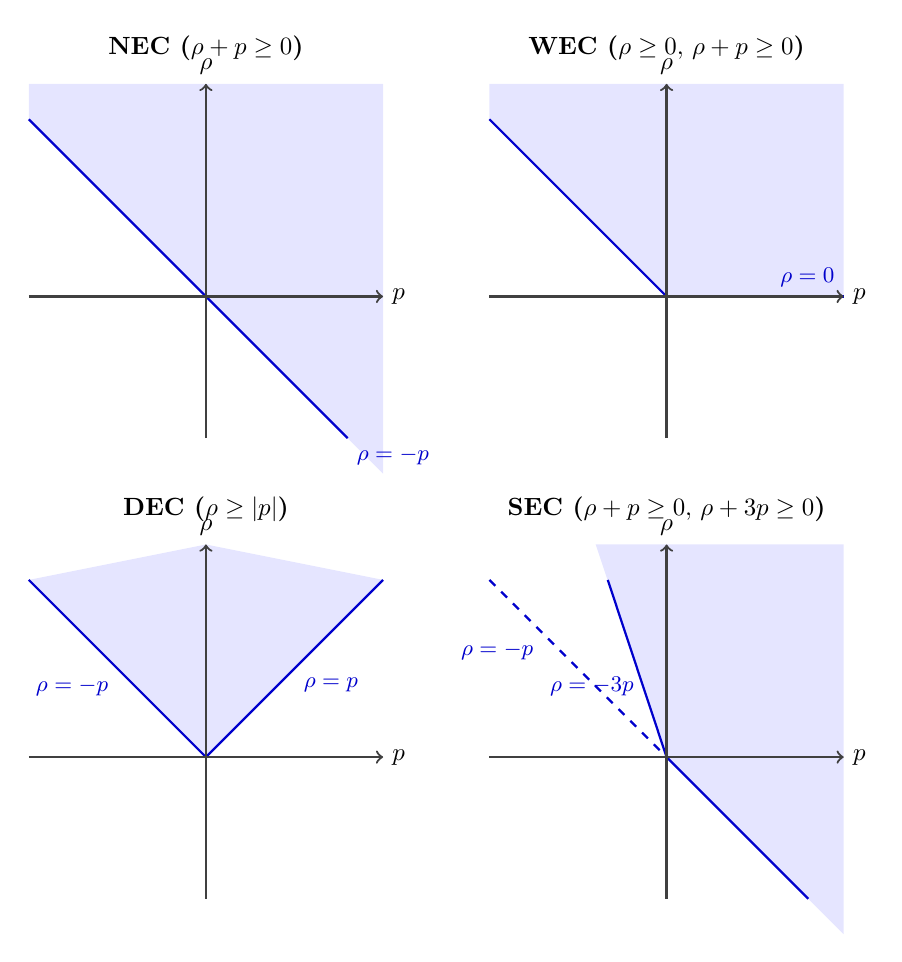
\begin{tikzpicture}[scale=0.9, every node/.style={scale=0.9}]
  % Common axes macro
  \def\drawaxes{
    \draw[->, thick, darkgray] (-2.5,0) -- (2.5,0) node[right, text=black] {$p$};
    \draw[->, thick, darkgray] (0,-2) -- (0,3) node[above, text=black] {$\rho$};
  }

  % NEC (Null Energy Condition)
  \begin{scope}[shift={(0, 6.5)}]
    \fill[blue!10] (-2.5, 2.5) -- (2.5, -2.5) -- (2.5, 3) -- (-2.5, 3) -- cycle;
    \draw[thick, blue!80!black] (-2.5, 2.5) -- (2.0, -2.0) node[below right, font=\small] {$\rho = -p$};
    \drawaxes
    \node[font=\bfseries] at (0, 3.5) {NEC ($\rho + p \ge 0$)};
  \end{scope}

  % WEC (Weak Energy Condition)
  \begin{scope}[shift={(6.5, 6.5)}]
    \fill[blue!10] (-2.5, 2.5) -- (0, 0) -- (2.5, 0) -- (2.5, 3) -- (-2.5, 3) -- cycle;
    \draw[thick, blue!80!black] (-2.5, 2.5) -- (0, 0);
    \draw[thick, blue!80!black] (0, 0) -- (2.5, 0) node[above left, font=\small] {$\rho = 0$};
    \drawaxes
    \node[font=\bfseries] at (0, 3.5) {WEC ($\rho \ge 0, \, \rho + p \ge 0$)};
  \end{scope}

  % DEC (Dominant Energy Condition)
  \begin{scope}[shift={(0, 0)}]
    \fill[blue!10] (0,0) -- (2.5, 2.5) -- (0, 3) -- (-2.5, 2.5) -- cycle;
    \draw[thick, blue!80!black] (-2.5, 2.5) -- (0, 0) node[midway, below left, font=\small] {$\rho = -p$};
    \draw[thick, blue!80!black] (0, 0) -- (2.5, 2.5) node[midway, below right, font=\small] {$\rho = p$};
    \drawaxes
    \node[font=\bfseries] at (0, 3.5) {DEC ($\rho \ge |p|$)};
  \end{scope}

  % SEC (Strong Energy Condition)
  \begin{scope}[shift={(6.5, 0)}]
    \fill[blue!10] (-1.0, 3) -- (0,0) -- (2.5, -2.5) -- (2.5, 3) -- cycle;
    \draw[thick, blue!80!black, dashed] (-2.5, 2.5) -- (0, 0) node[pos=0.3, below left, font=\small] {$\rho = -p$};
    \draw[thick, blue!80!black] (-0.83, 2.5) -- (0, 0) node[pos=0.6, left, font=\small] {$\rho = -3p$};
    \draw[thick, blue!80!black] (0,0) -- (2.0, -2.0);
    \drawaxes
    \node[font=\bfseries] at (0, 3.5) {SEC ($\rho + p \ge 0, \, \rho + 3p \ge 0$)};
  \end{scope}
\end{tikzpicture}
\caption{The four standard energy conditions in General Relativity.}
\label{fig:energy_conditions}
\end{figure}


% Drawing 5: Effective Potential for a Massive Particle
\begin{figure}[htbp]
\centering
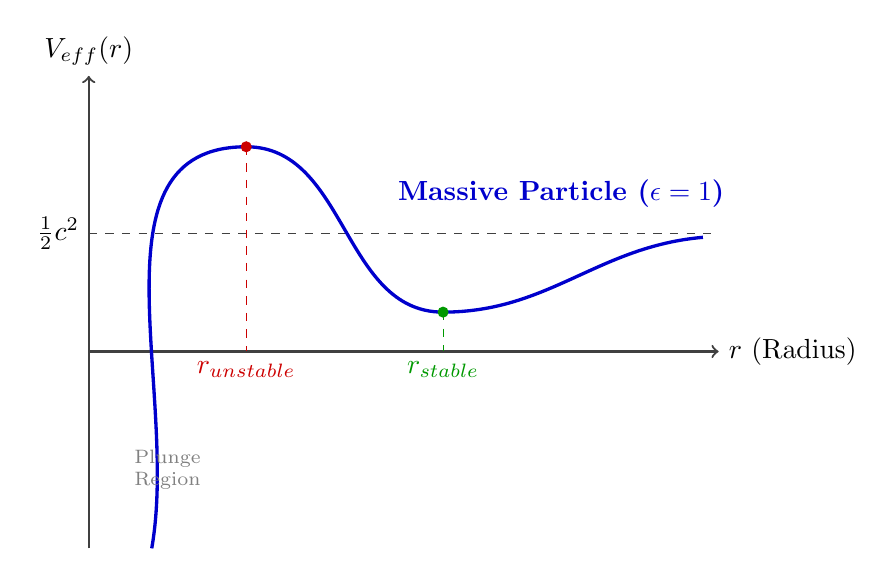
\begin{tikzpicture}[scale=1.0]
  % Axes
  \draw[->, thick, darkgray] (0,-2.5) -- (0, 3.5) node[above, text=black] {$V_{\text{eff}}(r)$};
  \draw[->, thick, darkgray] (0,0) -- (8, 0) node[right, text=black] {$r$ (Radius)};
  
  % Asymptote for massive particles (E_rest / m c^2)
  \draw[dashed, darkgray] (0, 1.5) node[left, text=black] {$\frac{1}{2}c^2$} -- (8, 1.5);

  % Extrema Coordinates
  \coordinate (Peak) at (2.0, 2.6);
  \coordinate (Min) at (4.5, 0.5);

  % The Effective Potential Curve (Massive Particle)
  \draw[very thick, blue!80!black] (0.8, -2.5)
    to[out=80, in=180] (Peak)
    to[out=0, in=180] (Min)
    to[out=0, in=185] (7.8, 1.45);
    
  % Annotations for Extrema
  \draw[dashed, red!80!black] (Peak) -- (2.0, 0) node[below] {$r_{\text{unstable}}$};
  \draw[dashed, green!60!black] (Min) -- (4.5, 0) node[below] {$r_{\text{stable}}$};
  
  \fill[red!80!black] (Peak) circle (2pt);
  \fill[green!60!black] (Min) circle (2pt);

  % Add a label for the curve
  \node[blue!80!black, font=\bfseries] at (6, 2.0) {Massive Particle ($\epsilon=1$)};
  
  % Singularity Region
  \node[align=center, font=\scriptsize, gray] at (1.0, -1.5) {Plunge \\ Region};
\end{tikzpicture}
\caption{Effective potential profile for a massive particle.}
\label{fig:effective_potential}
\end{figure}


% Drawing 6: Precession of Bound Orbits
\begin{figure}[htbp]
\centering
\begin{tikzpicture}[scale=1.0]
  \coordinate (O) at (0,0);

  % Orbit 1 (Initial)
  \begin{scope}[rotate=0]
    \draw[thick, blue!80!black, decoration={markings, mark=at position 0.65 with {\arrow{>}}}, postaction={decorate}] (1.5, 0) ellipse (2.5 and 1.8);
    \draw[dashed, red!80!black] (O) -- (-1, 0) coordinate (P1);
    \fill[red!80!black] (-1,0) circle (1.5pt);
  \end{scope}

  % Orbit 2 (Precessed)
  \begin{scope}[rotate=30]
    \draw[thick, green!60!black, decoration={markings, mark=at position 0.65 with {\arrow{>}}}, postaction={decorate}] (1.5, 0) ellipse (2.5 and 1.8);
    \draw[dashed, red!80!black] (O) -- (-1, 0) coordinate (P2);
    \fill[red!80!black] (-1,0) circle (1.5pt);
  \end{scope}
  
  % Orbit 3 (Further Precessed)
  \begin{scope}[rotate=60]
    \draw[thick, purple!70!black, decoration={markings, mark=at position 0.65 with {\arrow{>}}}, postaction={decorate}] (1.5, 0) ellipse (2.5 and 1.8);
    \draw[dashed, red!80!black] (O) -- (-1, 0) coordinate (P3);
    \fill[red!80!black] (-1,0) circle (1.5pt);
  \end{scope}

  % Central mass (Sun/Black Hole)
  \shade[inner color=yellow!90!white, outer color=orange!80!black] (O) circle (0.2) node[below=8pt, text=black, font=\bfseries] {$M$};

  % Precession angle arcs
  \draw[->, thick, red] (-0.7, 0) arc (180:210:0.5) node[midway, left=10pt] {$\Delta\phi$};
  \draw[->, thick, red] (-0.65, -0.375) arc (210:240:0.75) node[midway, left=10pt] {$\Delta\phi$};

  % Legend / Labels
  \node[blue!80!black, font=\small] at (4.5, 1.0) {Orbit $N$};
  \node[green!50!black, font=\small] at (3.5, 2.5) {Orbit $N+1$};
  \node[purple!80!black, font=\small] at (1.5, 3.8) {Orbit $N+2$};

\end{tikzpicture}
\caption{Orbital precession around a central mass.}
\label{fig:orbital_precession}
\end{figure}


% Drawing 7: Light Cones Narrowing (Schwarzschild Coordinates)
\begin{figure}[htbp]
\centering
\begin{tikzpicture}[scale=1.0]
  % Axes
  \draw[->, thick, darkgray] (0,-0.5) -- (0, 4.5) node[above, text=black] {$t$};
  \draw[->, thick, darkgray] (0,0) -- (6.5, 0) node[right, text=black] {$r$};

  % Horizon line
  \draw[ultra thick, dashed, red!80!black] (2.0, 0) -- (2.0, 4.5) node[above] {$r = 2GM$};
  
  % Singularity placeholder shaded area
  \fill[gray!20] (0,0) rectangle (2.0, 4.5);
  \node[rotate=90, gray, font=\small] at (1.0, 2.25) {Inside Horizon ($r < 2GM$)};

  % Light cones macro
  \newcommand{\schwarzschildcone}[3]{
    % #1: center x, #2: center y, #3: width (dt/dr slope factor)
    \begin{scope}[shift={(#1,#2)}]
      \fill[orange!20, opacity=0.8] (0,0) -- (-#3, 0.5) -- (#3, 0.5) -- cycle;
      \fill[orange!10, opacity=0.8] (0,0) -- (-#3, -0.5) -- (#3, -0.5) -- cycle;
      \draw[thick, orange!90!black] (-#3, -0.5) -- (#3, 0.5);
      \draw[thick, orange!90!black] (#3, -0.5) -- (-#3, 0.5);
      \fill[black] (0,0) circle (1pt);
    \end{scope}
  }

  % Draw light cones at different radii
  % As r -> 2GM, dt/dr -> infinity, so the cone becomes extremely narrow in space (x-width decreases)
  \schwarzschildcone{2.3}{2.2}{0.15}
  \schwarzschildcone{2.8}{2.2}{0.35}
  \schwarzschildcone{3.8}{2.2}{0.6}
  \schwarzschildcone{5.2}{2.2}{0.8}

  % Labels
  \node[font=\scriptsize, align=center] at (5.2, 3.0) {Flat Spacetime \\ Slopes ($\pm 45^\circ$)};
  \node[font=\scriptsize, align=center] at (2.4, 3.0) {Cones Severely \\ Narrow};

\end{tikzpicture}
\caption{Light cones narrowing near the horizon in Schwarzschild coordinates.}
\label{fig:lightcones_schwarzschild}
\end{figure}


% Drawing 8: Light Cones Tipping (Eddington-Finkelstein Coordinates)
\begin{figure}[htbp]
\centering
\begin{tikzpicture}[scale=1.3]
  % Axes
  \draw[->, thick, darkgray] (2.0,-0.5) -- (2.0, 5) node[above=10pt, text=black] {$v$ (Advanced Time)};
  \draw[->, thick, darkgray] (0,0) -- (7, 0) node[right, text=black] {$r$};

  % Singularity at r=0
  \draw[ultra thick, decorate, decoration={zigzag, segment length=6pt, amplitude=1.5pt}, red] 
    (0.5, 0) -- (0.5, 5) node[above, text=black] {$r = 0$};

  % Event Horizon
  \draw[ultra thick, dashed, blue!80!black] (3.0, 0) -- (3.0, 5) node[above] {$r = 2GM$};

  % Light Cones Macro for EF Coordinates
  \newcommand{\efcone}[4]{
    \begin{scope}[shift={(#1,#2)}]
      \fill[#4!20, opacity=0.8] (0,0) -- (0, 0.6) -- (#3, 0.6) -- cycle;
      \fill[#4!10, opacity=0.8] (0,0) -- (0, -0.6) -- (-#3, -0.6) -- cycle;
      \draw[thick, #4!90!black] (0, -0.6) -- (0, 0.6) node[pos=0.85, left, font=\tiny, text=black] {ingoing};
      \draw[thick, #4!90!black] (-#3, -0.6) -- (#3, 0.6);
      \fill[black] (0,0) circle (1.2pt);
    \end{scope}
  }

  % Outside Horizon
  \efcone{5.5}{2.5}{0.6}{orange}
  \node[font=\scriptsize, align=center] at (5.8, 3.4) {Far Outside:\\Escape Easy};

  \efcone{4.0}{2.5}{0.4}{orange}
  \node[font=\scriptsize, align=center] at (4.0, 3.4) {Approaching:\\Tipping Inward};

  % At Horizon
  \efcone{3.0}{2.5}{0.0}{red}
  \node[red!80!black, font=\scriptsize, align=center] at (3.0, 1.6) {At Horizon:\\Horizon is Null};

  % Inside Horizon
  \efcone{1.8}{2.5}{-0.35}{purple}
  \node[purple!80!black, font=\scriptsize, align=center] at (1.5, 3.6) {Inside:\\All Paths\\Lead to $r=0$};

\end{tikzpicture}
\caption{Light cones tipping inward in Eddington-Finkelstein coordinates.}
\label{fig:lightcones_eddington_finkelstein}
\end{figure}